\section{Ejercicio 7}
	Se pide experimentar con \texttt{SchedMistery}, y replicar su funcionamiento
	en \texttt{SchedNoMistery}.
	El scheduler funciona para un único core y puede tomar o no uno o más argumentos numéricos.

	\subsection{Análisis del scheduler}

	El mismo consiste en varias colas de prioridad cada una con un quantum
	asociado. Los quantums asignados a las colas de prioridad son de 1 quantum a la
	de máxima prioridad y los argumentos pasados por parámetro para las
	siguientes colas, de mayor a menor prioridad.

	Para entender el scheduler, se corrieron una serie de tareas.

	\begin{figure}[ht]
		\begin{center}
			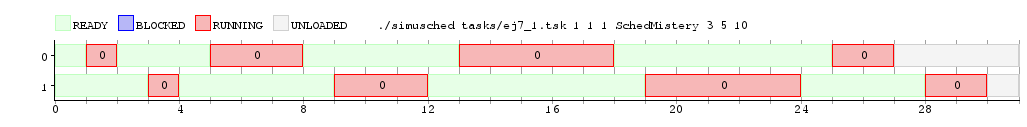
\includegraphics[width=1\columnwidth]{imagenes/ej7_1.png}
			\caption{Dos \texttt{TaskCPU} con 20 quantums.}
		\end{center}
	\end{figure}

	Se puede apreciar que cuando una tarea acaba sus quantums, es quitada de la
	cola donde está y es agregada en la siguiente cola de menor
	prioridad, si esto no es posible (está en la cola de pioridad mínima) queda
	donde está. Una vez que el scheduler desencola todas las tareas pendientes en una cola pasa a la siguiente.


	\begin{figure}[ht]
		\begin{center}
			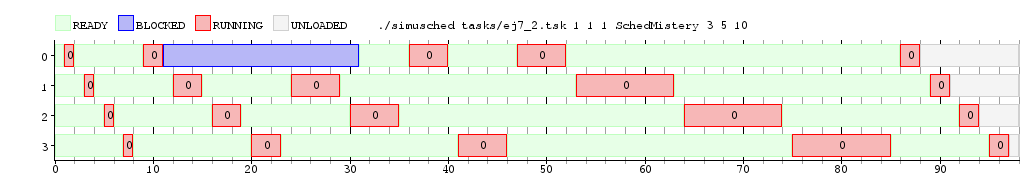
\includegraphics[width=1\columnwidth]{imagenes/ej7_2.png}
			\caption{Un \texttt{TaskCPU} corriendo con 20 quantums y tres
			\texttt{TaskAlterno} alternando 2 quantums de uso de CPU y 1 de bloqueo}
		\end{center}
	\end{figure}

	Como se puede apreciar este scheduler padece de inanición. Ocurre que las
	tareas con pocos o ningun bloqueo se acumulen en las colas con menor
	prioridad, mientras dos ó más tareas de mayor prioridad, se bloquen antes de
	que se les acabe el quantum, pasándose el control del CPU entre
	ellas.
	
	Cuando una tarea se desbloquea, es la próxima tarea a correr y su nivel de prioridad aumenta en uno.

	\begin{figure}[ht]
		\begin{center}
			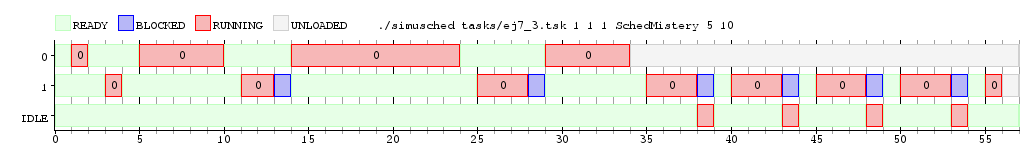
\includegraphics[width=1\columnwidth]{imagenes/ej7_3.png}
			\caption{Un \texttt{TaskCPU} corriendo con 20 quantums y un
			\texttt{TaskAlterno} alternando 2 quantums de uso de CPU, 1 de bloqueo al principio y después 4 y 2.}
		\end{center}
	\end{figure}

	\subsection{Implementación del Scheduler}

	\begin{itemize}
		\item \underline{Variables del Scheduler}
			\begin{itemize}
				\item \textbf{vq} : Es un vector de colas de enteros, la cola de enteros para guardar los pid de las tareas a correr y el vector de colas, una para cada prioridad.
				\item \textbf{def\_quantum} : Es un vector de enteros, donde se
					albergan los quantums asignados a cada prioridad.
				\item \textbf{unblock\_to}: Es un vector de enteros, donde cada proceso a través de su pid guarda su nivel de prioridad en el momento de su último bloqueo.
				\item \textbf{n} : Es un entero que indica en qué nivel de
					prioridad está corriendo el scheduler.
				\item \textbf{quantum} : Es un entero que indica cuántos ticks
					le queda a la tarea actual.
				\item \textbf{cur\_pri}: Es un entero que almacena el último pid que se acaba de desbloquear.
			\end{itemize}
		\item \underline{Funciones del Scheduler}
			\begin{itemize}
				\item \textbf{SchedNoMistery} : Toma los argumentos pasados por
					parámetro y se los asigna a def\_quantum, luego instacia las
					demás variables.
				\item \textbf{load}: Cuando una tarea entra en el scheduler es agregada en la cola en la cual está corriendo y es agregada en unblock\_to, por si en el futuro se bloquea.
				\item \textbf{tick} : Primero consulta si la tarea actual es la idle, ya que en ese caso se llama a \textbf{next} para saber quién será la próxima tarea a correr. En caso de no ser la tarea idle, si el motivo del tick es un \texttt{TICK} se procede de una
				manera y si es \texttt{BLOCK} de otra, mismo con \texttt{EXIT}.
				
				Si llega con motivo \texttt{TICK}, se decrementa en uno el
					quantum disponible, si le quedan quantums sigue la tarea
					actual, en caso contrario, la tarea que estaba corriendo es
					movida a la siguiente cola con menor prioridad si se puede,
					en caso contrario quedará en la cola donde pertenece (la de
					menor prioridad). Luego se llama a \textbf{next}, para saber
					quién sigue y por último se reinician los quantums correspondientes a la cola actual del scheduler.
				
				Si el motivo es \texttt{EXIT}, la tarea actual es desalojada dándole lugar a la próxima tarea llamando a \textbf{next} y reiniciando el quantum a su valor correspondiente a la cola actual del scheduler.
				
				Si el motivo es \texttt{BLOCK}, la tarea actual es desalojada dándole lugar a la próxima llamando a \textbf{next}, luego se almacena el nivel de prioridad subido en uno en unblock\_to y por último se reinicia el quantum a su valor correspondiente a la cola actual del scheduler.

				\item \textbf{next} : Debido a que saber quién es la proxima tarea a correr en el scheduler es una necesidad repetida se pasó a crear esta funcion.
				
				En caso que no haya ninguna tarea a correr, se devuelve la tarea idle.
				
				Si se desbloqueó una tarea se devuelve esa y el nivel de prioridad de scheduler pasa a ser el guardado en unblock\_to con su pid; caso contrario se busca a través de todas las colas, llendo de la prioridad actual a la menor, buscando la próxima tarea a ejecutar.

			\end{itemize}
	\end{itemize}




